\documentclass[]{article}  % list options between brackets
\usepackage{}              % list packages between braces
\usepackage{url}
\usepackage{listings}
\usepackage{graphicx}
\usepackage{color}
\usepackage{enumitem}



% type user-defined commands here

\begin{document}



\title{Real-Time Knowledge Management and Data-mining with Twitter}   % type title between braces
\author{Martin Moghadam, Kalle Grafstr\"{o}m}         % type author(s) between braces
\maketitle

\begin{figure}[h]
\centering

\includegraphics[scale=1]{Twitter_Icon.png}
\end{figure}

\begin{abstract}
Project in the course SSE3. Real-time tracking of human behavior on Twitter for survey, marketing and analysis. \\  The project focuses on Twitter for social network analysis, and the possibilities and exploits of using twitter as a data source for network analysis, exploring real-time analysis and analyzing a period of time. \\ Articles and research is examined and discussed, and a C\# client is developed for data gathering of Twitter streams. The client gathers the data, sorts and prepares the data for knowledge management, analysis of the knowledge collected is beyond the time and scope of this project. \\ Twitter has proven to be a very good source for social network analysis, because of the simple structure of the data and the ease of access. The data is freely available and the are no privacy concerns. Developing a C\# application is very straight forward with Web Services client model. \\ The application developed as a web service client could be expanded to gather data from other sources. Further development and knowledge management is discussed.

\end{abstract}





%=======================================
\section{Introduction}
Knowledge management used to identify and represent insights and experiences gained from data collected from Twitter, can prove useful in many circumstances. Some of which will be discussed in this article, others are left for further development, see discussion section. \\ The validity and credibility of the users identity is not discussed  in detail, we simply assume the user has a valid identity, see references for further details on "The Credibility of Digital Identity Information of the Social Web". \\ The project uses Twitter as a data source to comprise the knowledge, the Tweets all have dates and time allowing use to develop a systems that is updated minute by minute, gathering Information in real-time. This makes it possible to examine a period of time to extract knowledge from the Tweets in that period, for instance a debate performance\cite{bib10}.\\  The project work with the data gathering for the knowledge management, creating a Twitter traffic monitoring client application. \\ \\ We assume some prier experience with twitter is necessary to understand this article, the contents of tweets and the purpose of social network analysis is introduced.

	
\subsection{Twitter}
Twitter is a microblogging and social network service allowing users to send and read small text messages of up to 140 characters. The service has currently more than 100 million users worldwide. Users create accounts with profiles, the basic accounts are provided for free, premium account with a higher number of characters are purchasable. \\ The Tweets are associated to a specific user profile, the profile can have many followers that read the tweets. Each tweets has a time and date information, and can include; profile tags, topic tags and urls , this information can be used to structure and gain a greater understanding of the tweets. \newpage  The tweets contain different kinds for information as shown in figure \ref{figContent}. 

\begin{figure}[h]
\centering
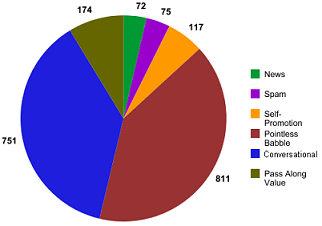
\includegraphics[scale=1]{Content_of_Tweets_Graphed.png}
\caption{Content of Tweets: Source Wikipedia}
\label{figContent}
\end{figure}
 

Searching the entire web for this kind of information would yield poor results because of the wast amount of trash data that needs to be sorted though. Such trash data is almost not present in Twitter. People commonly use Twitter to share information of what they are doing and where they are. Which included the geographical information on the user.\\ The knowledge we are interested in, is extracted from the conversational and pass along value data. The data from Twitter is available freely, and there are currently no privacy issues with gathering data. See figure \ref{figTweet} for an example of a tweet with; date, time and profile name.

\begin{figure}[h]
\centering
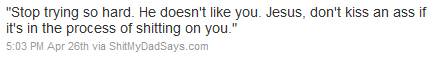
\includegraphics[scale=1]{tweet.png}
\caption{Example of a tweet with, date and time}
\label{figTweet}
\end{figure}

\subsection{Premise and Usage}
Twitter can and has been used to gather knowledge for:

\begin{itemize}
	\item Real-time recommendations for topical news. \cite{bib5}
	\item Marketing and research.
	\item Disaster monitoring, earthquakes, volcanoes, hurricanes. \cite{bib7}
	\item Political demonstrations. (The Iran demonstrations of 2009)
	\item Counter-terrorism.
	\item Many other possibilities.
\end{itemize}

A few people have used Twitter to make bomb treats, and encouraged assassination of politicians, these treats were not detected or monitored by an application, most of the threats were reported to the authorities by other users of the service but investigation  led to no results, because the threats were not serious just pointless babble. Generally people don't announce acts of terrorism on Twitter, and there has not been any evidence of a terrorists using Twitter, making it unsuitable for counter-terrorism. \\ Twitter already has been used for social network analysis some of which the results can be found in the references.

%=======================================
\section{Knowledge Management}
The knowledge management discipline we work with is social networks analysis, extracting data from the social networks and examining; likes dislikes, friendships, kinship, sexual relationships, beliefs, opinions, and connections to others. The interdependencies can be represented as nodes. \\ These nodes can be graphically represented (as shown in figure \ref{figGraph}, of all tweets with the \#GE2010 tag), the data providing a useful structured collection of knowledge. \\ 

\begin{figure}[h]
\centering
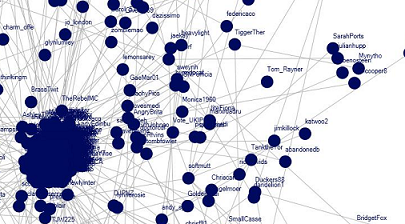
\includegraphics[scale=1]{twitter2010.png}
\caption{\#GE2010 Twitter Network Graph 3rd May 2010}
\label{figGraph}
\end{figure}

The knowledge can provide insight into;

\begin{itemize}
	\item Degree of separation between the users (Betweenness, Closeness).
	\item Ranking the users, Page Ranking.
	\item Ranking the Retweets (replays to a tweet).
	\item Ranking and discovering trends.
\end{itemize}

This knowledge management can provide insight into the trends and discussions of the entire Twittersphere, simply reading a few random tweets and following a few users won't do that.

\subsection{Real-time Knowledge}

In this case real-time means; computer system that update information at the same rate they receive information (data). The systems constantly monitors traffic, updating the data, since Twitter is a minute by minute system with time stamps, this is relatively  easy. When the data is updated in real-time the knowledge can update concurrently with the data, using a multi-thread application.

%=======================================
\section{Data Source}

For the development of the application we used C\# 4.0 and Visual Studio 2010, since we are already familiar with the development environment and the language, it was merely a choice of convenience, without much forethought.

\subsection{Twitter API and development}

Twitter provides an API (actually three APIs), which is entirely HTTP based, the API has limits to calls, follow requests, updates or direct message made each day. The API also has other limitation which will not be discussed here. \\ There are already a wast amount of libraries for Twitter, including libraries for languages like C++, C\# and Java. There are also a wast amount of open source clients. \\ For the educational project none of the libraries nor the Twitter API was used, but was used as a reference. The project was develop entirely as a  Web Services client using Dot Net.

\subsection{Twitter Streams}

Our application is designed to use one stream at a time, that means we gather data form one user or tag at a time. The application needs the stream to be define, for instance \url{http://twitter.com/OPRAH}, the application then gathers data from that user, for an entire data gathering of the Twittersphere, crawling is needed (like a web crawler), which is beyond the scope of our project.

\subsection{Code Example}

The code uses and is passed on and open source Twitter client. The client is a command-line client.The application was developed as a web service client based on HTTP.

\begin{figure}[h]
\centering
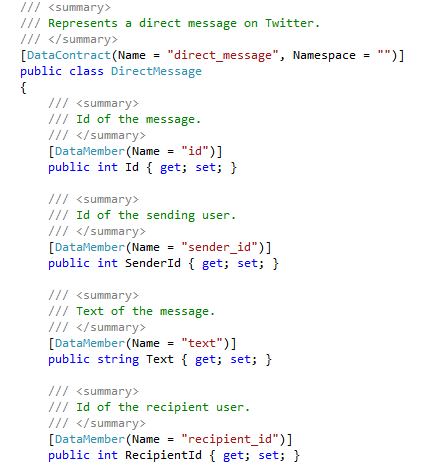
\includegraphics[scale=1]{code1.png}
\caption{Code exert}
\label{figCode1}
\end{figure}

The code exert in figure \ref{figCode1}, show the basic class of get, set method used for the client, the client does not use the set method but the were kept for further development, only get methods are used to gather the data and serialize it into a text file. The data is sorted according to time and date, and some basic search and sort was attempted to extract knowledge from the data, no graphical interface or representation of the knowledge was created.\\ Due to time constraints no further sorting or knowledge extraction is performed, and no further details of the client is discussed.

\subsection{Test and Development}

No substantial test was preformed, and the development was modifying the acquired code to simplify the application and to customize it for our project. 


%=======================================       
\section{Discussion}

The Twitter social network analysis has great potential to monitor and gather information on human behavior and the premise we started with was validated, further development is discussed. 

\subsection{Further Development}

Creating a more complete application of social network analysis for Twitter is possible for further development. The application could be a web app, were the user could define a period of time for analysis then the application would search and collect data from Twitter. \\ The application could be improved to included the following features;

\begin{itemize}
	\item Twitter stream crawling, gather data from the entire Twittersphere.
	\item Betweenness, Closeness, Measures in social network analysis.
	\item Relationship detection, using the tag and link information to determine interdependencies.
	\item Geographic information gathering.
	\item Node Structuring, using the detected interdependencies to form a large node structure of the social network.
	\item Graphical representation, showing the interdependencies as nodes making the relationship and connection clear and easy to understand.
	\item Identity Credibility, create a identity credibility system to improve the accuracy of the interdependencies.
	\item Multi-treading and distributed solution for mass real-time Twitter social network analysis. Twitter is big and getting bigger, to analysis such a system in real-time a scalable application is needed.
\end{itemize}

\subsection{Conclusion}

A solution to extract data for Twitter was found and some basic analysis was test, making it a good starting point for a more complex Twitter social network analysis application. Such a project could be expanded to collection knowledge for other social networks like Facebook. Gaining another 400 million user accounts to monitor, making that a total of approximately 550 million accounts to monitor and analysis.

% Creates entry in bibliography even if it isn't cited.
\nocite{bib1} 
\nocite{bib2}
\nocite{bib3}
\nocite{bib4}
\nocite{bib5}
\nocite{bib6}
\nocite{bib7}
\nocite{bib8}
\nocite{bib9}
\nocite{bib10}
\nocite{bib11}
\nocite{bib12}
\nocite{bib13}



\bibliographystyle{unsrt} % references appear in order of citations
\bibliography{references}

\end{document}